
\section{Inteligencia artificial, \textit{Machine Learning}, \textit{Deep Learning} y Inteligencia Artificial Generativa}

Comencemos por describir las diferentes disciplinas que intervienen en el estudio y desarrollo de sistemas de inteligencia artificial. A menudo se encuentran términos como \glsdisp{ia}{Inteligencia Artificial (IA)}, \glsdisp{ml}{\textit{Machine Learning} (ML)}, \glsdisp{dl}{\textit{Deep Learning} (DL)} e, incluso, \glsdisp{iag}{Inteligencia Artificial Generativa (IAG)}, usados de forma intercambiable. Sin embargo, cada uno tiene un significado específico, y es crucial diferenciarlos para comprender el estado actual de la investigación en el área. Estos conceptos se organizan jerárquicamente \citep{torresivinalsPythonDeepLearning2020}, donde la  \gls{ia} es el término más general, que abarca el \gls{ml}, y este último incluye al \gls{dl} y la gls{iag} (ver Figura \ref{fig:ai_ml_dl_gai}).

\begin{figure}[H]
    \caption[Relación entre Inteligencia Artificial, \textit{Machine Learning}, \textit{Deep Learning} y \textit{Generative AI}]{Relación entre Inteligencia Artificial, \textit{Machine Learning}, \textit{Deep Learning} e Inteligencia Artificial Generativa}
    \centering
    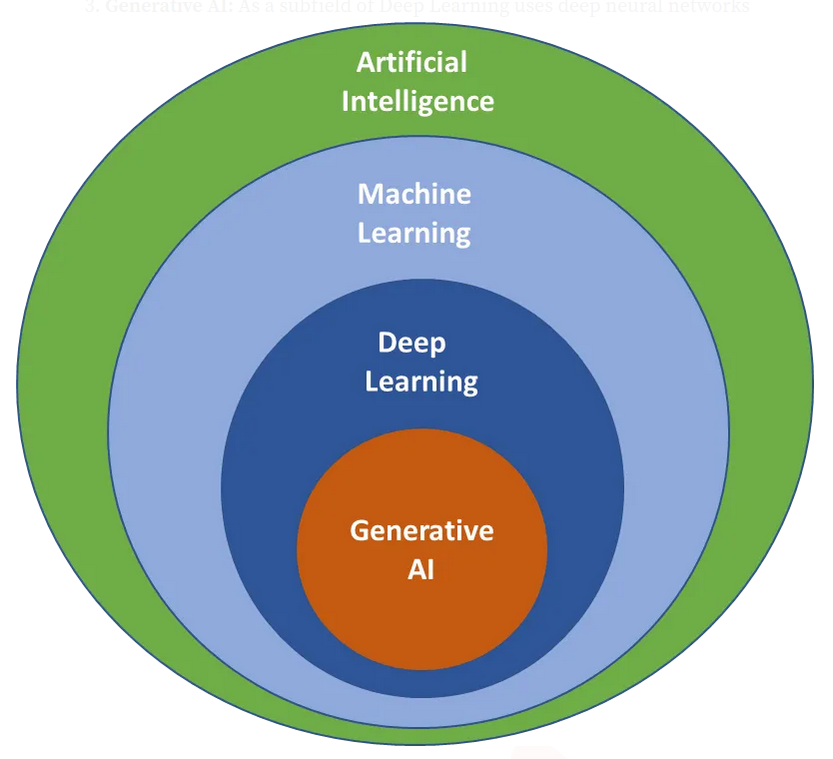
\includegraphics[width=0.5\textwidth]{./figuras/ai_ml_dl_gai.png}
    \source{\cite{kainatIntroductionGenerativeAI2023}}
    \label{fig:ai_ml_dl_gai}
\end{figure}

La \gls{ia}, como concepto genérico, es el campo de estudio más antiguo entre los tres, y no se limita únicamente al ámbito computacional. En su sentido más amplio, la \gls{ia} ha sido abordada por la filosofía. Los racionalismos y estructuralismos, fundamentales en los sistemas de pensamiento occidentales, forman la base conceptual de la \gls{ia}. Sin embargo, no es hasta el siglo XX cuando se empieza a considerar la posibilidad matemática de un sistema que genere inteligencia. En 1950, Alan Turing publicó su artículo \textit{Computing Machinery and Intelligence} \citep{alan1950a}, en el que propuso un test para determinar si una máquina puede pensar. Este test, conocido como <<test de Turing>>, consiste en la interacción de un humano con una entidad artificial usando solo un terminal de texto como interfaz. La máquina pasa el test si el humano no puede discernir si está interactuando con una entidad artificial o humana. A pesar de sus limitaciones y su enfoque antropocéntrico sobre la inteligencia, este test sigue siendo una referencia común para evaluar sistemas modernos de \gls{ia}.\todo{Buscar una referencia de utilización de test de Turing actualmente}

No obstante, el concepto de \gls{ia} trasciende a la mera imitación de lo humano. Si consideramos la <<racionalidad>> como un conjunto de estructuras lógicas que incluyen el pensamiento y el entendimiento humanos, la \gls{ia} no necesita limitar su objetivo a superar el test de Turing. Las definiciones de \gls{ia} a lo largo del tiempo han variado dependiendo de si se enfocan en imitar el pensamiento o acción <<humanos>> o el pensamiento y acción <<racional>> \citep{RussellStuartJ2021AI:A}.

% Además de a Alan Turing, debemos a Curt Gödel los fundamentos matemáticos de los procesos de pensamiento, considerados sistemas computacionales capaces de generar \textit{outputs} racionales a partir de \textit{inputs} arbitrarios. 

La idea de que el cerebro humano es una de las posibles <<máquinas de Turing>> \citep{penroseNuevaMenteEmperador2015} ha sido un estímulo para la investigación en \gls{ia} computacional. Además, investigaciones en <<procesamiento del lenguaje natural>>, en las que destaca el concepto de <<entropía>> de Shannon \citep{shannon1951prediction} y que han acompañado el desarrollo de lenguajes de programación, son fundamentales para los sistemas actuales de \gls{ia}. \todo{Explicar brevemente los conceptos de máquita de Turing y de entropía en este contexto, fundamental para comprender el funcionamiento de los modelos de lenguaje. Es importante ser breve\dots}


\subsection{\textit{Machine Learning}}

El  \glsdisp{ml}{\textit{Machine Learning}}, o \textit{aprendizaje automático}, es una rama de la \gls{ia} que investiga algoritmos y modelos matemáticos que habilitan a un sistema computacional a aprender a partir de datos sin ser explícitamente programado. Estos sistemas identifican patrones y toman decisiones con poca o sin intervención humana. En el \gls{ml}, el sistema se autoconfigura basándose en los datos con los que se entrena. Las únicas intervenciones humanas son el diseño de la arquitectura y la provisión de los datos de entrenamiento, aunque incluso estas tareas podrían delegarse a otro sistema de \gls{ml} en determinadas circunstancias.

Aunque el \gls{ml} ha sido una área de interés desde los inicios de la computación, es esencial reconocer que es solo una faceta de la \gls{ia}. No todos los sistemas inteligentes son sistemas de \gls{ml}. Como ejemplo, el software de ajedrez \textit{Deep Blue} de IBM, que venció al campeón mundial Garry Kasparov en 1997, no se basaba en \gls{ml} \citep{campbellDeepBlue2002}. En lugar de ello, \textit{Deep Blue} utilizaba una vasta base de datos de jugadas de ajedrez y algoritmos de búsqueda heurísticos para decidir el mejor movimiento en cada situación. Otros sistemas no basados en \gls{ml}, como los <<sistemas expertos>>, utilizan reglas predefinidas para tomar decisiones y se aplican ampliamente en áreas como medicina, ingeniería o gestión empresarial.

En términos generales, el objetivo del \gls{ml} es encontrar funciones matemáticas que describan un conjunto de datos de entrenamiento y que, posteriormente, pueda ser utilizada para prever datos desconocidos con precisión. Esta capacidad predictiva se conoce como <<inferencia>>. El proceso busca que la función determinada durante el entrenamiento se aproxime lo más fielmente posible a la función real que describe los datos. Modelos complejos y grandes, pueden llegar a generalizar de forma análoga al cerebro humano. 


Se utiliza el término <<modelo>> para referirse al sistema una vez que ha sido entrenado y posee capacidad predictiva. Dependiendo de su aplicación, un modelo puede ser empleado para predecir datos desconocidos o clasificarlos. Si produce un valor numérico, se habla de <<regresión>>; si categoriza datos, de <<clasificación>>. La clasificación puede ser binaria o multiclase, y la regresión unidimensional o multidimensional. La Figura \ref{fig:ml_classification_regression} muestra un ejemplo de clasificación y regresión.\todo{Si se encuentra alguna imagen buena para esto, ok, si no, exponer de otro modo la información para que se entienda.}

\missingfigure[figwidth=.4\textwidth]{Añadir: ejemplo de clasificación y regresión}
\label{fig:ml_classification_regression}

El aprendizaje en \gls{ml} se produce a través de un proceso de entrenamiento. Según la naturaleza de los datos y el método de validación, existen tres tipos principales de aprendizaje automático \citep[p. ~38]{torresivinalsPythonDeepLearning2020}:

\begin{itemize}
    \item \textbf{Aprendizaje supervisado:} Aquí, los datos se etiquetan con la respuesta esperada, como imágenes de animales etiquetadas como <<gato>> o <<perro>>. Tras el entrenamiento, se espera que el sistema identifique imágenes no etiquetadas correctamente. Este procedimiento de aprendizaje e inferencia queda reflejado en la Figura \ref{fig:labeled_data_training}. Una de las aplicaciones más comunes del aprendizaje supervisado es la clasificación de imágenes. Sin embargo, su debilidad consiste precisamente en la necesidad de etiquetado de los datos de entrenamiento, que puede ser un proceso costoso y laborioso si este solo se puede hacer manualmente.
    
    \item \textbf{Aprendizaje no supervisado:} En este caso, los datos no están etiquetados. El sistema busca patrones y agrupa datos en categorías por sí mismo. Precisamente este es el tipo de aprendizaje utilizado en el entrenamiento de modelos de lenguaje, donde los datos de entrenamiento son textos sin etiquetar.
    
    \item \textbf{Aprendizaje por refuerzo:} El sistema aprende interactuando con un entorno. No recibe etiquetas explícitas, sino recompensas por decisiones correctas y penalizaciones por errores. Este es el modo de aprendizaje más parecido al humano, ya que se basa en la experiencia. Sin embargo, a pesar de ser uno de los métodos más atractivos de aprendizaje automático, es el más complejo de implementar y requiere un entorno de simulación adecuado, que no siempre es posible ni eficiente en términos de computación.
\end{itemize}

\begin{figure}[H]
    \caption[Esquema de aprendizaje supervisado]{Esquema de aprendizaje supervisado, usando datos de entrenamiento etiquetados. En la inferencia se espera que el modelo pueda clasificar datos no etiquetados.}
    \centering
    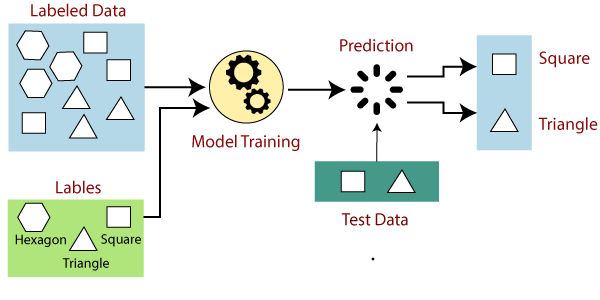
\includegraphics[width=0.6\textwidth]{./figuras/labeled_data_training.png}
    \source{\cite{FindWaysDeal}}
    \label{fig:labeled_data_training}
\end{figure}


\subsection{\textit{Deep Learning}}

Esta sección pretende ser una somera introducción a los conceptos de \glsdisp{dl}{\textit{Deep Learning}} o <<Aprendizaje Profundo>> y \gls{rna}, que constituyen la base de los modelos de lenguaje, objeto de nuestro estudio, con la única finalidad de aportar un aparato teórico mínimo en el que contextualizarlo. En los últimos meses la bibliografía sobre este tema está creciendo exponencialmente. Además de las obras citadas en este trabajo, se puede consultar, a modo de introducción para no especialistas, \cite{BeginnerGuideNeural}. El \gls{dl} es una rama del \gls{ml} que utiliza redes neuronales artificiales para aprender de forma automática. Las \gls{rna} son modelos matemáticos cuyos principios imitan el funcionamiento de las neuronas biológicas y hunden sus raíces en la intersección entre biología, matemáticas y ciencias de la computación ya en la primera mitad del siglo XX.

\subsubsection{El concepto de neurona artificial}

Para entender en qué consiste una \gls{rna} y, por extensión, de un modelo de \gls{dl}, antes es necesario comprender el concepto de <<neurona artificial>>. Una neurona artificial no es sino un modelo simplificado de una neurona natural que encontramos en el sistema nervioso de los animales. Análogamente a su homóloga biológica, una neurona artificial recibe una serie de valores de entrada, los procesa y devuelve una salida. La entrada de una neurona artificial es la suma ponderada de las salidas de las neuronas de la capa anterior. Esta suma ponderada se pasa a una función de activación, que determina la salida de la neurona. Sin necesidad de entrar en detalles matemáticos, la función de activación más común es la función sigmoide, que devuelve un valor entre 0 y 1 de una forma no lineal. La Figura \ref{fig:neurona_artificial_natural} muestra un esquema de una neurona artificial. \todo{Explicar brevemente el procedimiento del funcionamiento a partir de la imagen. Estaría bien conceptualizarla con su fórmula matemática, quizás la única fórmula del trabajo...}

\begin{figure}[H]
    \caption[Neurona biológica y neurona artificial o <<perceptrón>>]{Neurona biológica y neurona artificial o <<perceptrón>>}
    \centering
    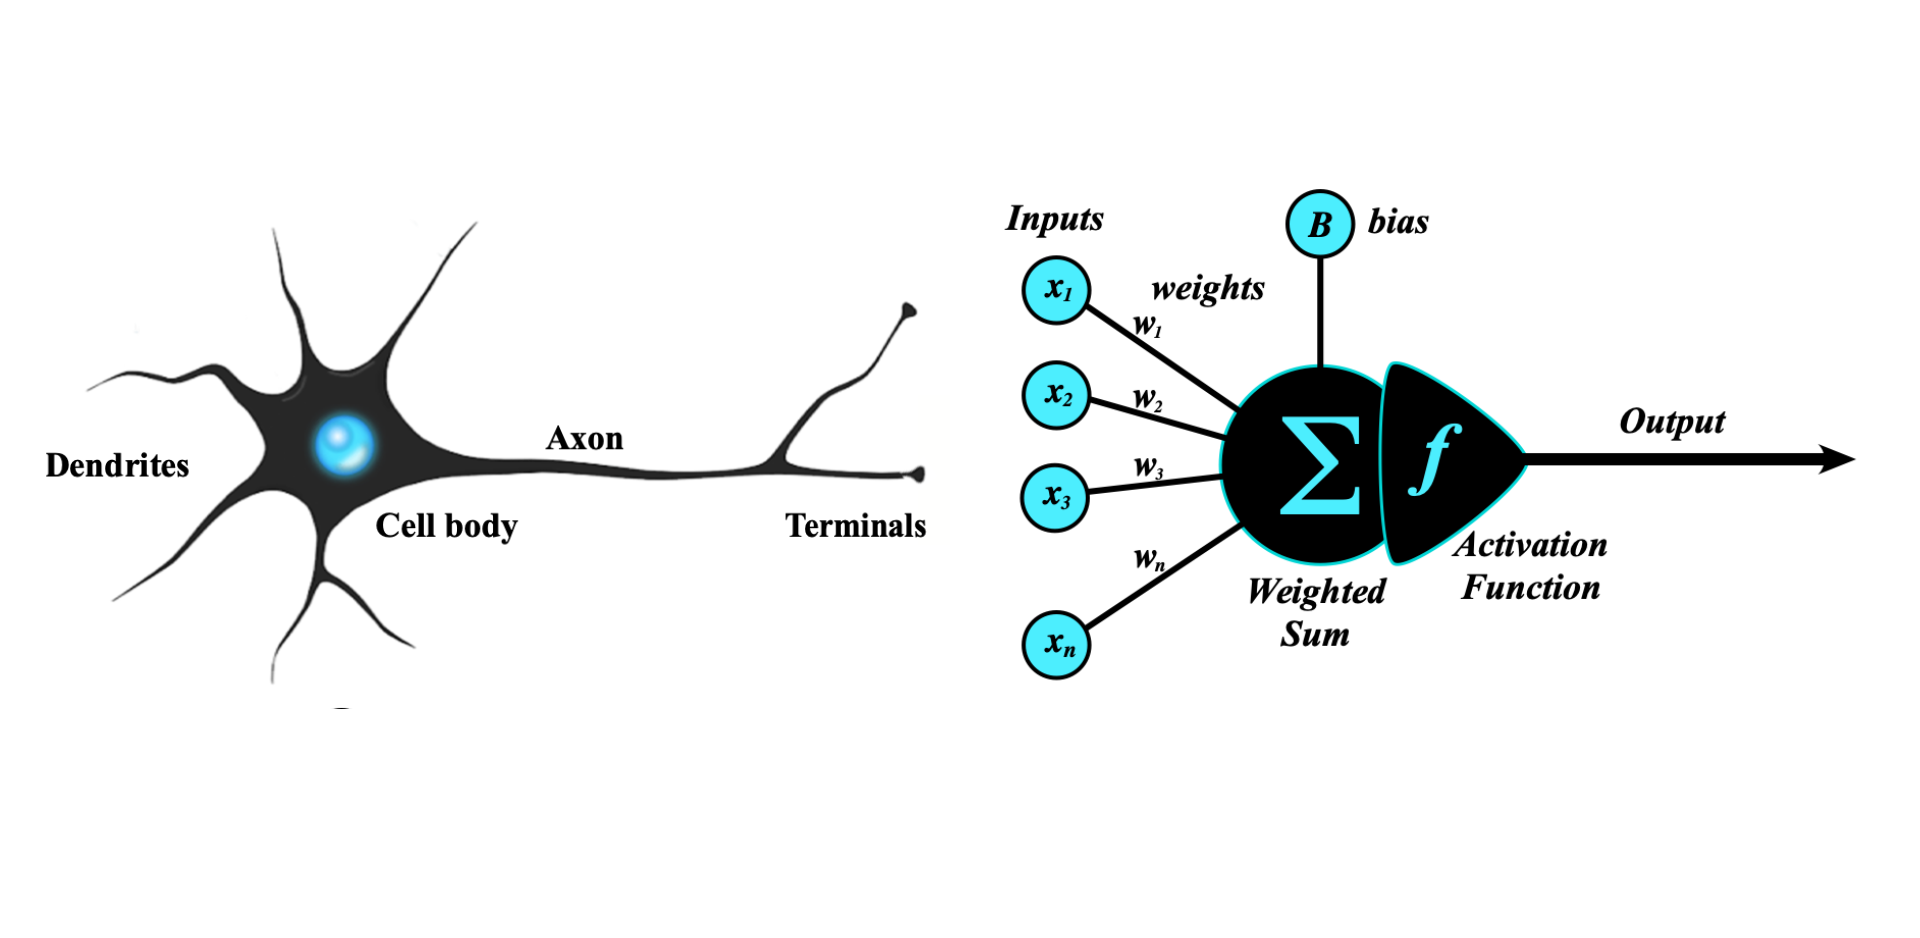
\includegraphics[width=0.5\textwidth]{./figuras/perceptron_with_neuron.png}
    \source{\cite{DeepLearningDL}}
    \label{fig:neurona_artificial_natural}
\end{figure}

El concepto de <<neurona artificial>> fue expuesto por primera vez por F. Rosenblatt en 1958 \citep{rothmanTransformersNaturalLanguage2021} bajo el nombre de <<perceptrón>>. El perceptrón no es otra cosa que un modelo de clasificación binaria, es decir, que solo puede clasificar datos en dos categorías. Rosenblatt planteó su modelo para ser implementado en \textit{hardware}, y, de hecho, se construyó un prototipo en 1959. Sin embargo, el perceptrón tenía ciertas limitaciones matemáticas que no permitían su aplicación a problemas más complejos. En 1969, Minsky y Papert publicaron el libro \citep{minsky1969perceptrons}, en el que demostraban que el perceptrón no podía resolver problemas linealmente no separables. Este hecho supuso un freno en la investigación en \gls{rna}, que no se retomó hasta la década de los 80, cuando se desarrollaron nuevos modelos de redes neuronales artificiales que permitían resolver problemas más complejos que un simple perceptrón. 

Actualmente sabemos que una red neuronal de varias capas puede aproximar arbitrariamente cualquier función matemática, lo que ha venido a llamarse <<teorema de la aproximación universal>>, propuesto en 1989 por Hornik en su artículo \textit{Multilayer Feedforward Networks Are Universal Approximators} \citep{hornikMultilayerFeedforwardNetworks1989}. Este teorema tiene grandes implicaciones, no solo científicas, sino también filosóficas, en la medida en que podemos considerar que una \gls{rna} es capaz de imitar el funcionamiento del cerebro humano y su comportamiento, el cual puede reducirse al de una función matemática por compleja que esta sea. En otras palabras, este teorema afirma que existe una <<máquina de Turing>> capaz de modelar el cerebro humano. R. Penrose (\citeyear{penroseNuevaMenteEmperador2015}) explora las implicaciones de que nuestro cerebro fuera una <<máquina de Turing>>.\todo{Aquí se hace nueva ref a la máquina de Turing, razón de más para explicarla bien más arriba}


\subsubsection{Redes neuronales artificiales}
Una \gls{rna} es un modelo matemático que se compone de varias capas de neuronas artificiales. La primera capa se denomina <<capa de entrada>> y recibe los datos de entrada. La última capa se denomina <<capa de salida>> y devuelve la predicción del modelo. Las capas intermedias se denominan <<capas ocultas>> y son las que permiten que el modelo pueda aproximar cualquier función matemática. La Figura \ref{fig:deep_neural_network} muestra un esquema de una \gls{rna} con una capa de entrada, dos capas ocultas y una capa de salida.

% La salida de la neurona se pasa a las neuronas de la capa siguiente, y así sucesivamente hasta llegar a la capa de salida. La salida de esta última capa es la predicción del modelo. 

\begin{figure}[H]
    \caption[Estructura de capas de una red neuronal artificial]{Estructura de capas de una red neuronal artificial, con una capa de entrada, dos capas ocultas y una capa de salida.}
    \centering
    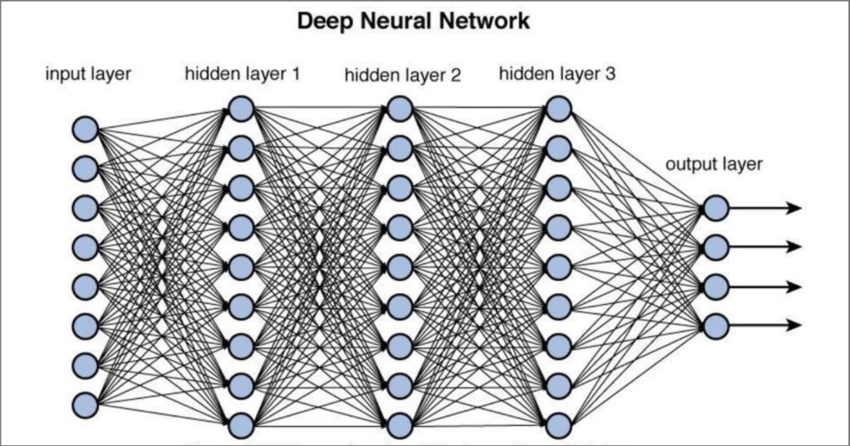
\includegraphics[width=0.6\textwidth]{./figuras/Deep_neural_network.png}
    \source{\cite{zraraPORTFOLIOOPTIMIZATIONUSING2021}}
    \label{fig:deep_neural_network}
\end{figure}

En función de los objetivos de la \gls{rna}, su arquitectura o estructura interna puede variar considerablemente. Una \gls{rna} puede constar de una sola capa, de una capa de entrada y otra de salida y de múltiples capas ocultas. Cada arquitectura busca resolver un tipo de problema concreto. Una arquitectura especialmente compleja, y que ha dado muy buenos resultados en la visión artificial es la \gls{cnn}, inspirada en el funcionamiento de la corteza visual del cerebro humano. Las \gls{cnn} se utilizan para el reconocimiento de imágenes y vídeos, y han sido la base de los avances en el campo de la visión artificial en los últimos años.

Independientemente de su estructura, una \gls{rna} o modelo de \textit{Deep Learning} debe ser entrenado a partir de los datos, de los cuales <<aprende>>. El proceso de entrenamiento consiste en presentar los datos de entrenamiento a la \gls{rna} y ajustar sus parámetros internos para que la salida se aproxime a la salida esperada. Este proceso se repite iterativamente hasta que la salida de la \gls{rna} se aproxima a la salida esperada con un margen de error aceptable. Una vez entrenada, la \gls{rna} puede predecir la salida de datos desconocidos. Este proceso se ilustra en la Figura \ref{fig:ann_training} Por parámetros internos entendemos los pesos de las conexiones entre neuronas, que son los que en definitiva determinan la salida de la \gls{rna}. Un modelo antes de ser entrenado da como salida valores aleatorios, y el entrenamiento consiste en ajustar estos valores para que la salida se aproxime a lo esperado. Existe una relación, grosso modo, entre la cantidad de parámetros (pesos) de un modelo y su capacidad predictiva, al tiempo que aumenta considerablemente el tiempo de entrenamiento y la capacidad computacional necesaria para entrenarlo. Esta es una de las razones por las que ha habido que esperar a los últimos años para empezar a ver resultados comparables a los del cerebro humano, en tareas generativas de imágenes, vídeo, audio o texto.

\begin{figure}[H]
    \caption[Diagrama de entrenamiento de una red neuronal artificial]{Diagrama de entrenamiento de una red neuronal artificial.}
    \centering
    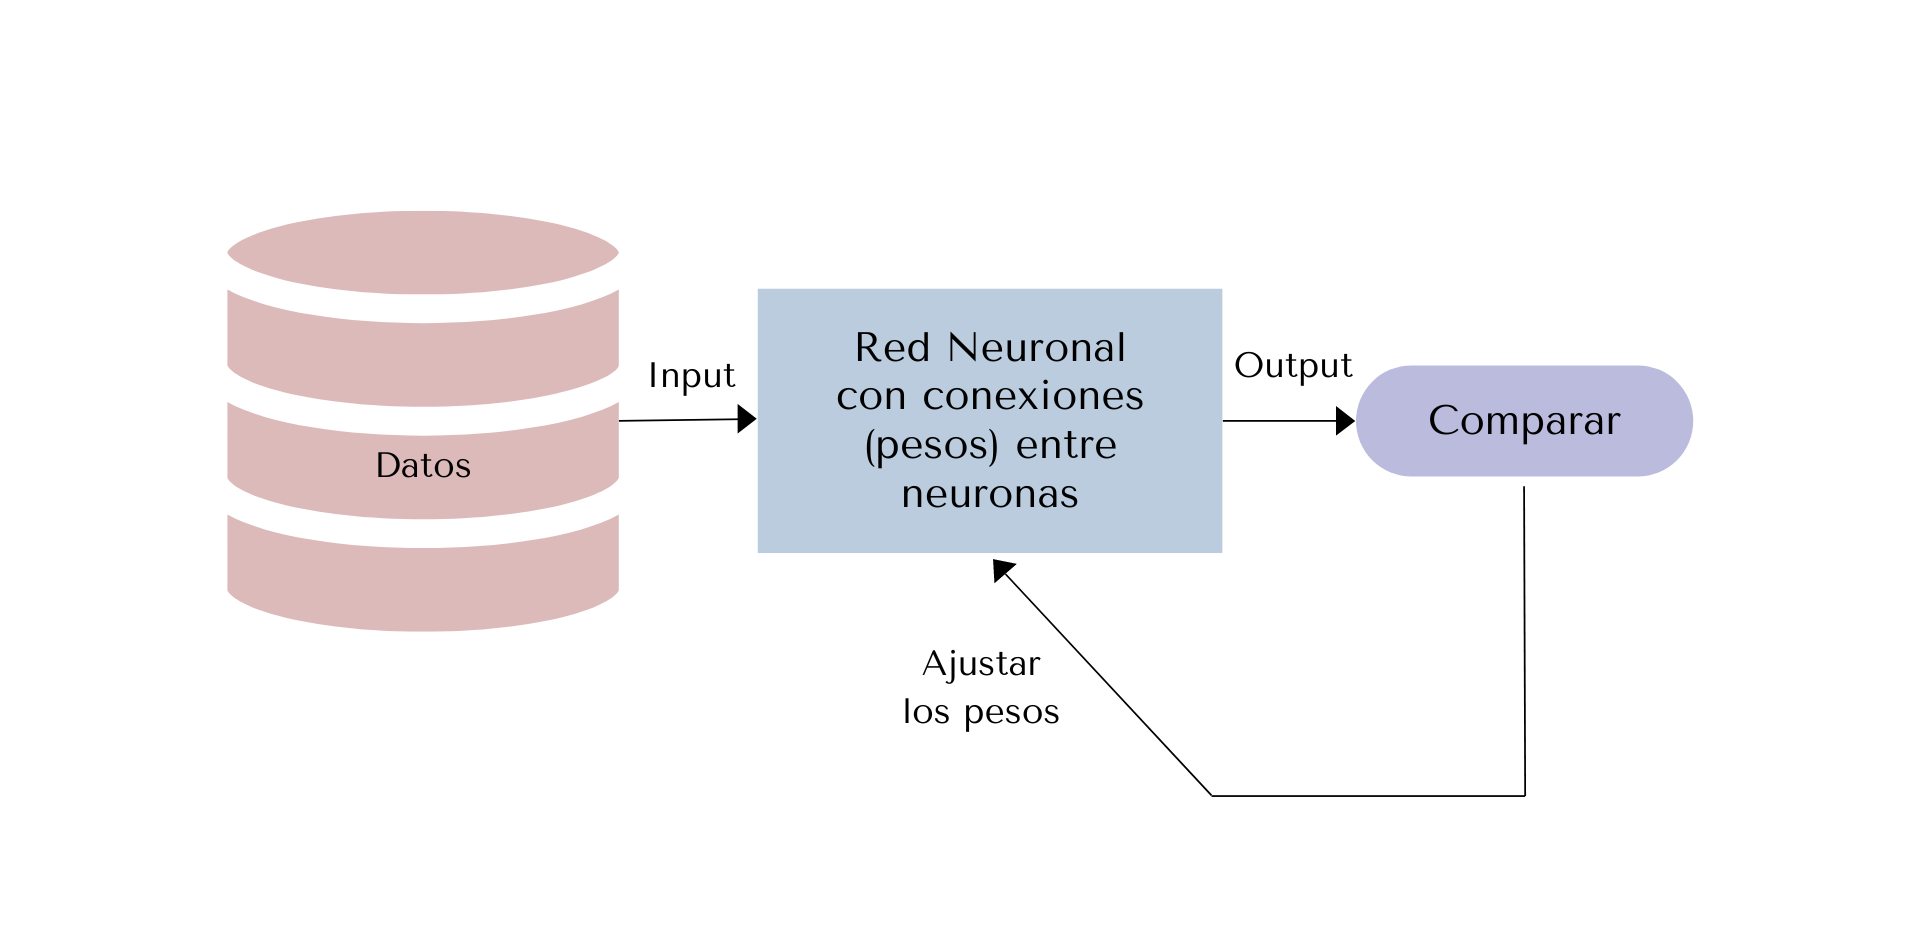
\includegraphics[width=0.9\textwidth]{./figuras/ann_training.png}
    \source{Elaboración propia}
    \label{fig:ann_training}
\end{figure}

\subsubsection{Redes neuronales recurrentes}
Hasta 2017, el estado del arte en el ámbito del procesamiento de lenguaje natural por medio de modelos de \gls{dl} eran las redes neuronales recurrentes (RNN). Estas se basaban en la idea de que la salida de una neurona se podía retroalimentar a la entrada, de forma que la salida de la neurona en el instante $t$ se podía usar como entrada en el instante $t+1$. Esta arquitectura se ilustra en la Figura \ref{fig:red_neuronal_recurrente}. Sin embargo, las RNN presentaban un problema conocido como \textit{vanishing gradient}, que hacía que el modelo no pudiera retener contextos de secuencias largas, ya que su <<atención>> se desvanece en los \textit{tokens}\todo{poner en pie de página la definición de token} más alejados en el tiempo. Este problema se solucionó en parte con las redes neuronales de memoria a corto y largo plazo (LSTM), que permitían que la información fluyera a través de la red sin perderse. Sin embargo, las LSTM no podían trabajar con grandes cantidades de \textit{tokens} de contexto, lo que limitaba su aplicación a tareas de procesamiento de lenguaje natural.

\begin{figure}[H]
    \caption[Arquitectura de una red neuronal recurrente]{Arquitectura de una red neuronal recurrente.}
    \centering
    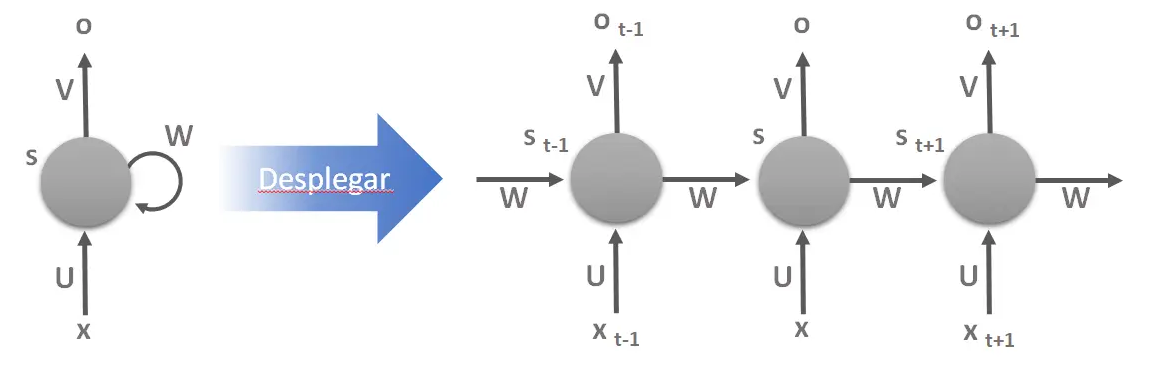
\includegraphics[width=0.9\textwidth]{./figuras/red_neuronal_recurrente.png}
    \source{\cite{calvoRedNeuronalRecurrente2018}}
    \label{fig:red_neuronal_recurrente}
\end{figure}


\subsubsection{La arquitectura \textit{Transformer}}
En junio de 2017, \citeauthor{vaswaniAttentionAllYou2017} publicaron un artículo \citep{vaswaniAttentionAllYou2017} en el que proponían una nueva arquitectura de red neuronal, denominada \textit{Transformer}, que no se basaba en las RNN y que permitía trabajar con grandes cantidades de \textit{tokens} de contexto. Esta arquitectura se basaba en el concepto de \textit{atención}, que permite que el modelo pueda aprender de secuencias largas. En esta arquitectura, no importa la posición de los \textit{tokens} de la secuencia de entrada, ya que el modelo aprende a asignar pesos a cada \textit{token} en función de su relevancia para la predicción del siguiente \textit{token}. A diferencia de una RNN, un \textit{Transformer} puede procesar todos los \textit{tokens} de una secuencia de entrada en paralelo, lo que lo hace mucho más eficiente computacionalmente tanto en el entrenamiento como en la inferencia. La Figura \ref{fig:transformer_attention} muestra una matriz de atención de un \textit{Transformer} entrenado con textos en inglés.

En la figura \ref{fig:transformer_architecture} se puede ver el esquema de la arquitectura \textit{Transformer} tal como se presentó originalmente en \textit{Attention is All You Need} \cite{vaswaniAttentionAllYou2017}.

\begin{figure}[H]
    \caption[Aquitectura de Transformer]{Aquitectura de Transformer. Esta imagen se ha convertido en icono de la revolución de la IA generativa.}
    \centering
    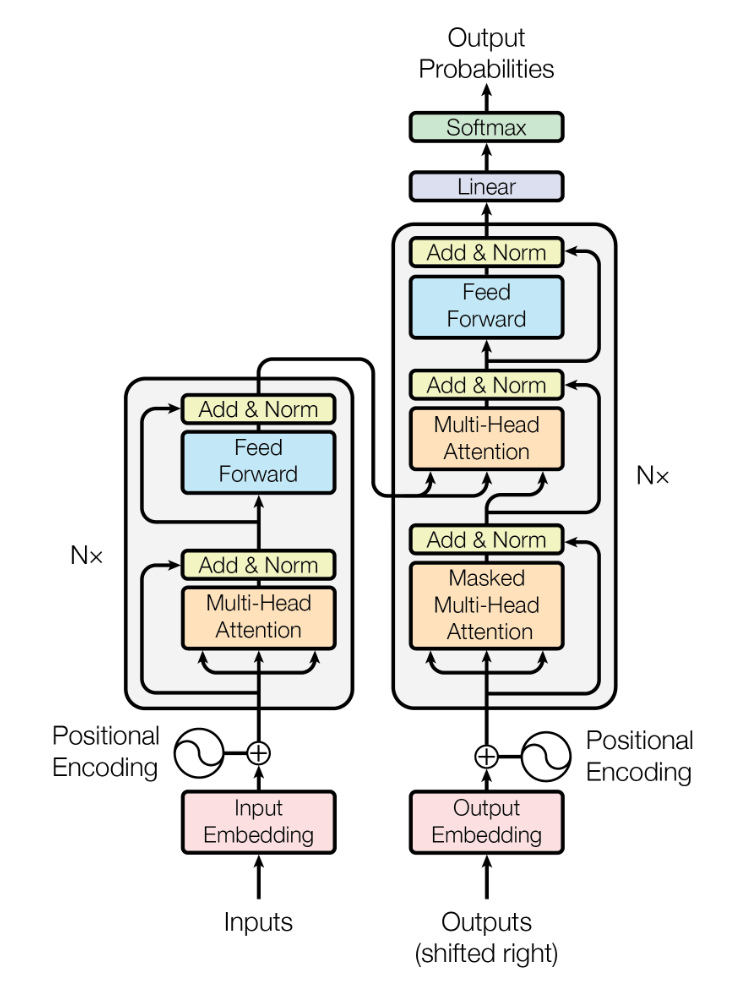
\includegraphics[width=0.4\textwidth]{./figuras/Transformer_architecture.png}
    \source{\cite{vaswaniAttentionAllYou2017}}
    \label{fig:transformer_architecture}
\end{figure}

\begin{figure}[H]
    \caption[Matriz de \textit{atención} de un \textit{Transformer} entrenado con textos en inglés]{Matriz de \textit{atención} de un \textit{Transformer} entrenado con textos en inglés. En ella queda representada la atención de cada token de la secuencia de entrada <<He later went to report Malaysia for one year>> con respecto a los demás.}
    \centering
    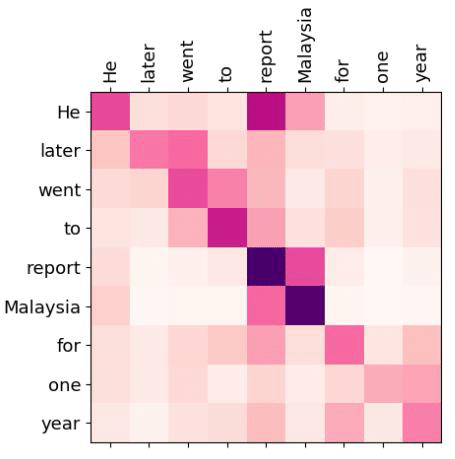
\includegraphics[width=0.4\textwidth]{./figuras/Transformer_attention_matrix.png}
    \source{\cite{duAddressingSyntaxBasedSemantic2022}}
    \label{fig:transformer_attention}
\end{figure}

\subsection{Inteligencia artificial generativa}\todo{Explicar brevemente en qué consiste la IAG: generación de imágenes, vídeo, audio, texto, etc.}
